\begin{exercise}
  Lösen Sie das Hamilton System aus Example 6.4 des Vorlesungsskriptes
  numerisch mit den RK4 Verfahren aus Example 2.25, der impliziten
  Mittelpunktsregel aus Example 3.5 und einem symplektischen
  Eulerverfahren aus Example 6.29. Beobachten Sie die
  Hamilton-Funktion der numerischen Lösung für lange Zeiträume.
  Erklären Sie die Ergebnisse.
\end{exercise}

\begin{solution}
\begin{figure}
    \centering
    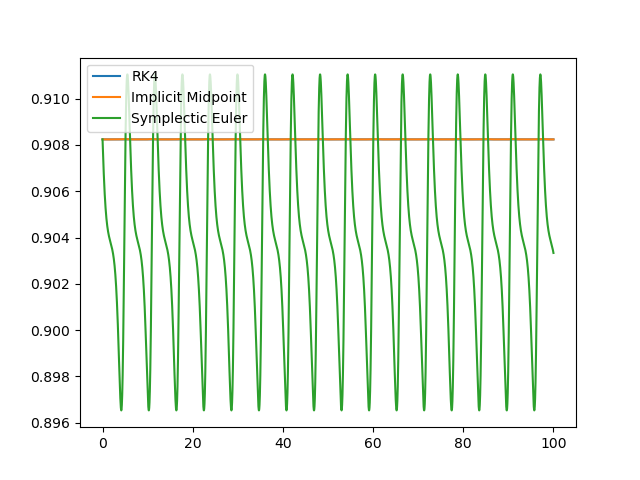
\includegraphics[width=\linewidth]{plot47neu.png}
\end{figure}
\FloatBarrier
\end{solution}
